\chapter{Background} % nothing of mine

utrolig mye bra her: https://www.dei.unipd.it/\~emg/downloads/SIMPAR08-WorkshopProceedings/TeachingWithRobotics/karatrantou.pdf!! veldig mange bra kilder \hfill \\

og mange eksempler herfra: https://student.cs.uwaterloo.ca/~cs231/resources/pseudocode.pdf \hfill \\

mer på pseudokode: https://www.researchgate.net/profile/Nicholas-Bennett-6/publication/309410533\_Introduction\_to\_Algorithms\_and\_Pseudocode/links/60a489d04585158ca05c54bc/Introduction-to-Algorithms-and-Pseudocode.pdf \hfill \\

This chapter will cover concepts that one should be familiar with in order to fully understand the rest of this thesis. We start by providing a definition for pseudocode, to avoid confusion further down the line, as well as discussing transpiling, why Haskell is a good tool for the job, and how other transpilers work.

\section{Pseudocode}

Pseudocode is a technique for describing computer programs in a more abstract way than programming languages allow, ignoring specific syntax and keywords. This can make programs easier to understand for both non-programmers and programmers alike, particularly when working with unfamiliar algorithms \cite{LinfoAlgorithmsIntro2007}. \hfill \\

Since it does not follow exact syntax rules of any kind, pseudocode is subsequently not executable. This is not a bug, but rather a feature of pseudocode: it is intended for presenting ideas of code, not demonstrating results of code [kilde?]. As such, pseudocode is an abstract concept, and can technically be anything, as long as it aims to aid others in understanding what a particular piece of code does. \hfill \\

Usually, pseudocode is used at a more granular level, describing \textit{parts} of a problem, rather than the entire problem itself [kilde?]. For instance, when presenting a solution to a group of non-technical people, presenting pseudocode of the entire project is not necessarily enlightening. Alternatively, presenting the programs core, or other pieces of code directly related to the programs core, might provide valuable insight to people who can come with suggestions for improvement, despite not being able to program it themselves. \hfill \\

Now, since pseudocode has many faces, we must define what we percieve pseudocode to be in the context of this thesis, and what exactly we mean when we refer to ``pseudocode'' in later parts of the thesis. To avoid further confusion, we will make a distinction between two particular types of pseudocode: text based- and image based pseudocode.

\subsection{Text based pseudocode}

The most common form of pseudocode is likely text based pseudocode (TBP), commonly found in text books on algorithms, published papers, as well as informal scribbling before attempting to solve a problem \cite{payAttentionToMLPs}\cite{BOOK:intro/Cormen/Leiserson}. It is also the form that most closely resembles source code, given that it usually includes line numbers, assign statements and generally presents the problem solution in an imperative matter \cite{proposalForParadigmGeneralPseudocode}. \hfill \\

Since there is no proper set of rules commanding how text based pseudocode should look like, we are prone to viewing different variations of the same algorithms across different literatures. A frequently presented algorithm is Binary Search, which in the context of computer science is a search algorithm that finds the position of a target value within a sorted array \cite{BOOK:intro/Cormen/Leiserson}. \hfill \\

Here is how it is presented in The Design and Analysis of Computer Algorithms by Aho et al. in 1974 \cite[139]{BOOK:DesignAnalysis/Aho}:

\begin{lstlisting}
    procedure SEARCH(a, f, l):
    if f $>$ l then return "no"
    else
        if a = A[$\lfloor$(f + l)/2$\rfloor$] then return "yes"
        else
            if a < A[$\lfloor$(f + l)/2$\rfloor$] then
                return SEARCH(a, f, $\lfloor$(f + l)/2$\rfloor$ - 1)
            else return SEARCH(a, $\lfloor$(f + l)/2$\rfloor$ + 1, l)
\end{lstlisting}

Then, roughly 17 years later, Lewis et al. present it like this in Data Structures and Their Algorithms \cite[182]{BOOK:DSA/Lewis}:

\begin{lstlisting}[basicstyle=\small\ttfamily]
    function BinarySearchLookUp(key K, table T[0..n-1]): info
    {Return information stored with key K in T, or $\Lambda$ if K is not in T}
        Left $\gets$ 0
        Right $\gets$ n - 1
        repeat forever
            if Right < Left then
                return $\Lambda$
            else
                Middle $\gets$ $\lfloor$(Left + Right) / 2$\rfloor$
                if K = Key(T[Middle]) then return Info(T[Middle])
                else if K < Key(T[Middle]) then Right $\gets$ Middle - 1
                else Left $\gets$ Middle + 1
\end{lstlisting}

The desire for automatic generation of TBP has been in the wind for some time, with the intention of presenting ideas without having to worry about syntax of a particular programming language \cite{desireToGetPseudocodeGeneration}. Text based pseudocode allows authors to draft ideas in an imperative way, just like we write recipes for baking bread and building legos. Here, the author is free to omit boilerplate code, include mathematical notation and necessary abstractions, and even resort to natural language where deemed appropriate \cite{BOOK:intro/Cormen/Leiserson}\cite{DBLP:conf/els/Nuallain15}. \hfill \\

As such, we can comfortably regard the succinctness of figure 2.1 displaying TBP, to figure 2.2 displaying an implementation of said TBP in a popular programming language \cite{javaIsAPopularProgrammingLanguage}:

\begin{figure}[ht]
    \centering
    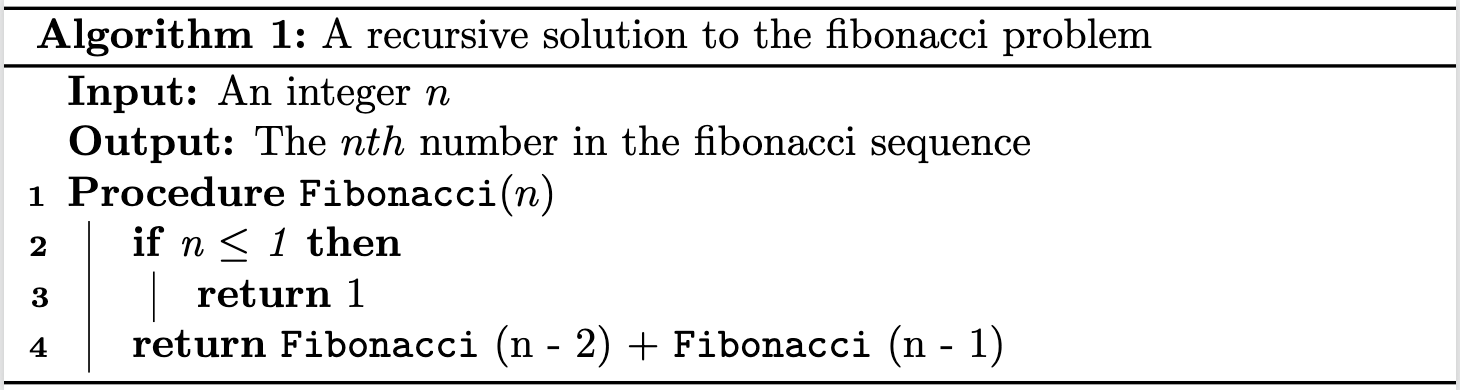
\includegraphics[scale=0.46]{assets/fibonacci_pseudo1.png}
    \caption{Text based pseudocode illustrating an algorithm to retrieve the nth number in a fibonacci sequence.}
    \label{fig:fibseq1}
\end{figure}

\begin{figure}[ht]
    \centering
    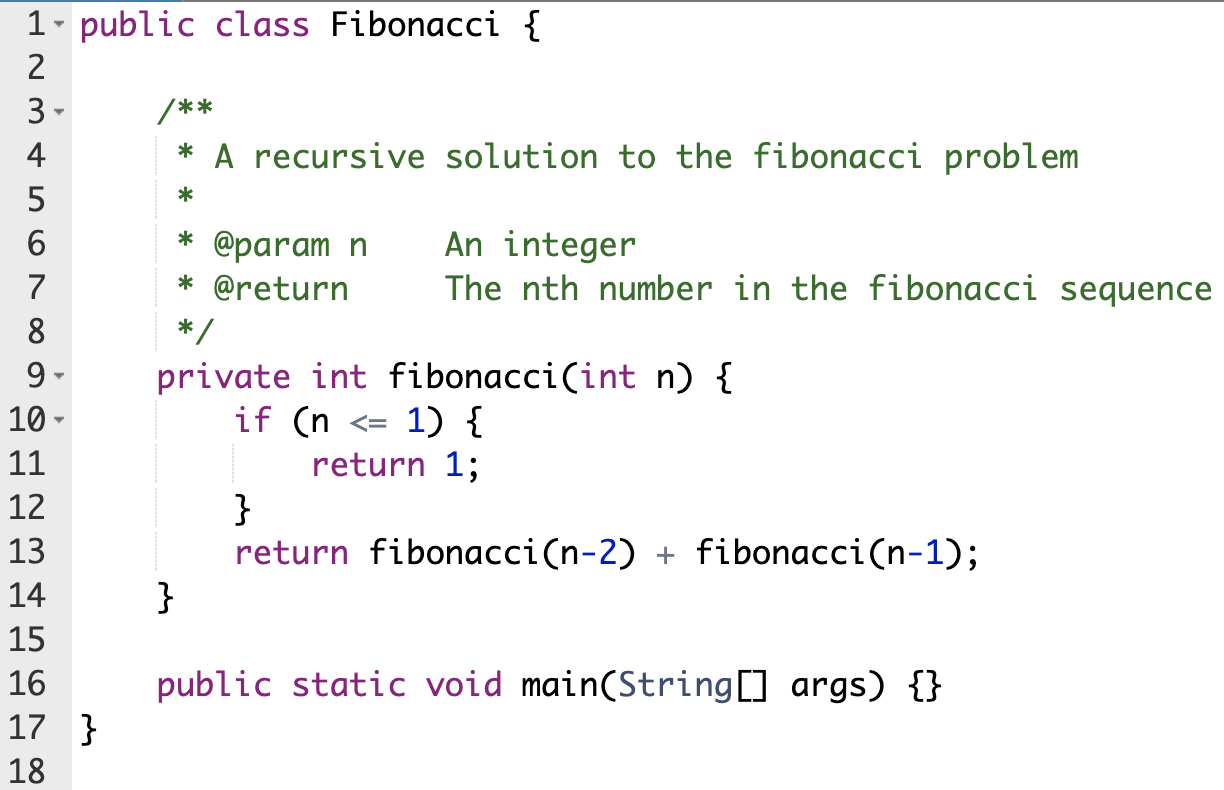
\includegraphics[scale=0.50]{assets/fibonacci_java.png}
    \caption[An algorithm written in the Java programming language, to retrieve the nth number in a fibonacci sequence.]{An algorithm written in the Java programming language, to retrieve the nth number in a fibonacci sequence. It follows the commenting guidlines JavaDoc\footnotemark.}
    \label{fig:fibjava}
\end{figure}
\footnotetext{https://docs.oracle.com/javase/8/docs/technotes/tools/windows/javadoc.html}

It is a useful tool when wanting to discuss unpolished ideas with friends and colleagues, but as mentioned, it has a rich history of being applied in university curriculums too. When learning algorithms, datastructures, or programming concepts in general, the concepts tend to be more important than the specific implementation details in the author’s programming language of choice. Thus, it can be advantageous for students to learn with TBP rather than source code, as we are keeping the style similar, but not demanding familiarity with a particular programming language. \hfill \\

Its usefulness is also backed by the numerous attempts at translating source code to TBP in the past \cite{PSEU:/Kreher/Stinson}\cite{DBLP:conf/kbse/OdaFNHSTN15}\cite{DBLP:conf/aswec/AlhefdhiDHG18}.

\subsection{Image based pseudocode}

Not all programming languages share the same execution flow. For istance, in VHDL all processes are executed simultaneously\footnote{https://www.people.vcu.edu/~rhklenke/tutorials/vhdl/modules/m12\_23/sld008.htm}, whilst rewriting rules in Maude are applied in an arbitrary order [kilde]. Some, on the other hand, like Python, will execute their programs line for line. This means that we can follow the execution flow simply by looking at the order functions are called and the order of statements within those functions. \hfill \\

This way of executing a program opens up for the possibility of image based pseudocode (IBP), which still includes text, but also complements it with boxes, arrows and perhaps pretty colours. When code stretches over enough lines, it all starts looking similar and confusing. IBP, on the other hand, does a good job of isolating each statement, and potentially gives more of a birds eye view perspective of the code. \hfill \\

In fact, images in computer science is nothing new. One of the most notable examples we have are the ones we use for finite state automata (FSA). An FSA is a machine which either accepts or rejects a given string, by running each symbol through a state sequence uniquely determined by said string. We differentiate betwee deterministic and non-deterministic FSAs, though it is not of importance in our context. What they share, is a number of states, a start state, a transition function and an accept state \cite{introToAutomataTheory}.

\begin{figure}[ht]
    \centering
    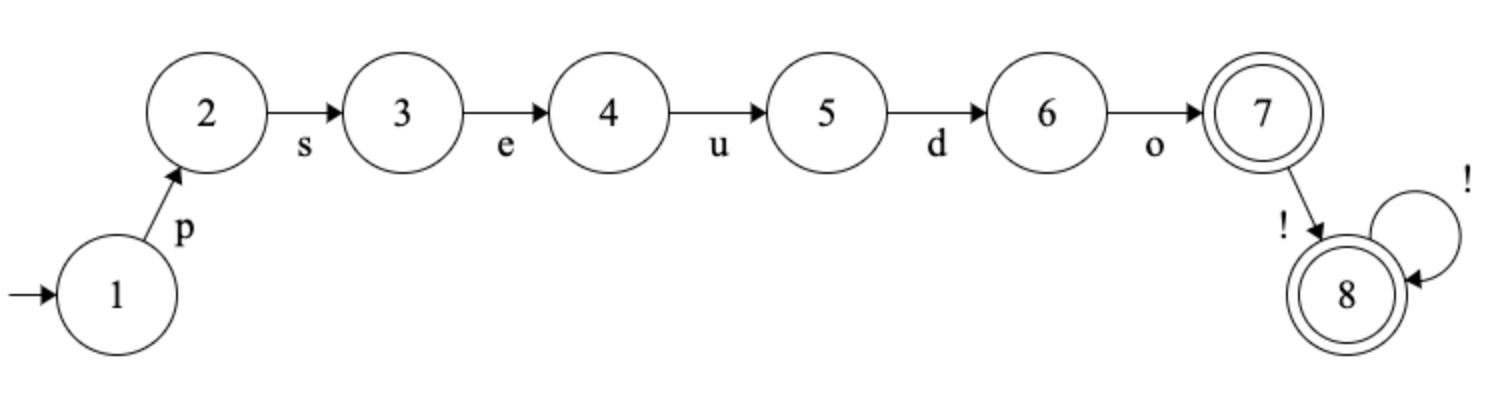
\includegraphics[scale=0.46]{assets/dfa.png}
    \caption{An example finite state automata.}
    \label{fig:dfa}
\end{figure}

Figure 2.3 shows an example of an FSA which accepts the word ``pseudo'' followed by 0 or more exclamation marks. The FSA has 8 states, and the leftmost arrow indicates that state 1 is the starting state. From here, we can get to the second state if our string starts with the symbol ``p''. Thus, all strings that do not begin with a ``p'' are rejected at this point. States 7 and 8 have an additional ring within their circle, which means that they are accepting states. If a combination of symbols have not been rejected at this point, and is finished, it is accepted. State 8 has an arrow leading to itself via the symbol ``!'', meaning that it can end with as many exclamation marks as possible. \hfill \\

A string like ``pseudo!!p!!!'' is not accepted, however, because despite starting with ``pseudo!!'' and ending with ``!!!'', once a string has reached state 8 it can \textit{only} be followed by exclamation marks, or else it is instantly rejected. \hfill \\

Warren McCulloch and Walter Pitts were among the first researchers to introduce a concept similar to finite automata, all the way back in 1943 \cite{McCulloch43}. Their paper presents a simplified computational model of biological neurons. \hfill \\

Throughout the remainder of this thesis, when we talk about ``image based pseudocode'', we are referring to flowcharts. The title does not technically belong to flowcharts alone, but it is the way we will go about things. \hfill \\

There have also been multiple attempts at creating flowchart editors, most notably by Carlisle et al. and Charntaweekhun et al. \cite{carlisle2004}\cite{charntaweekhun2006}. These allows authors to visualise their ideas, rather than keeping it all text based. Benefits of learning with help from visual aid is well documented, which is one of the reasons introductory math books are always so colourful [kilde?]. It seems a stretch to believe that students could not benefit from learning with images also when it comes to algorithms and programming concepts. \hfill \\

\begin{figure}[ht]
    \centering
    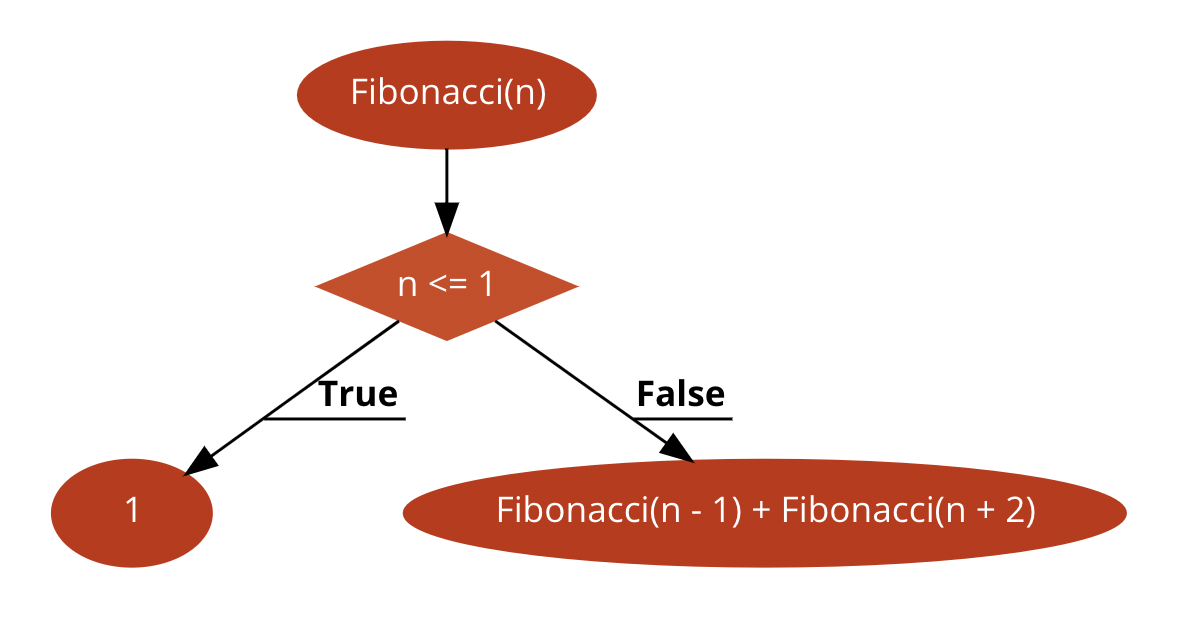
\includegraphics[scale=0.46]{assets/fibonacci_flowchart.png}
    \caption{Image based pseudocode illustrating an algorithm to retrieve the nth number in a fibonacci sequence, created with Code2Flow.}
    \label{fig:fibseq1}
\end{figure}

Given the imperative nature of flowcharts, the way they walk through problems step-by-step, it should not be impossible to convert image based psueodcode back to text based pseudocode. In fact, this has been attempted by Wu et al., with positive results \cite{codeFromFlowcharts}. This gives even more ground to perceive flowcharts as an image based form of pseudocode. \hfill \\

There have been multiple studies documenting the preference for IBP when it comes to studying algorithms, already back in the 80s by Scanlan et al. He documented how his students overwhelmingly preferred structured flowcharts to pseudocode for comprehending algorithms. Using multiple algorithms of varying complexity, the students most notably indicated that the flowcharts took less time to comprehend, provided fewer errors in understanding, and reduced the number of times they had to look at the algorithms \cite{DBLP:journals/software/Scanlan89}. \hfill \\

In newer times, Nita et al. attempted to analyse student's understanding of algorithms with pseudocode and flowcharts. The students were subjected to algol-like TBP, and IBP. Their conclusion was that the students found it easier to understand the selected algorithms in image format, as compared to a text based approach \cite{Nita_2020}.

% Bra språk for å snakke om flowcharts: https://www.researchgate.net/publication/234805404_Flowchart_techniques_for_structured_programming

\section{Transpiling}

A transpiler is a tool that converts input source code into output source code, maintaining an approximate abstraction level \cite{DBLP:conf/els/MarcelinoL22}. For instance, the first transpiler to our knowledge was developed in 1978 by Intel, with the aim of translating assembly source code from the 8080/8085 processor to the 8086 processor \cite{intel1979}. \hfill \\

An alternative to transpiling is the well-known phenomenon of \textit{compiling}. The difference is that we do not stay on the same abstraction level, but rather we make it much more specific. An example of this is compiling a Java file to bytecode. To humans, the bytecode reads like the most foreign language, though the JVM understands it perfectly, and is able to execute it[kilde?]. \hfill \\

A hot example of transpiling involves the JavaScript programming language\footnote{https://developer.mozilla.org/en-US/docs/Web/JavaScript/Language\_overview}, commonly used in web development. It is a language in constant development, frequently updating its features. The issue with this is that not all browsers are always compatible with its newest features. Therefore, there exists a transpiler Babel\footnote{https://babeljs.io} which converts modern JavaScript into a backwardcompatibla version. According to Nicolini et al., without a transpiler almost 14\% of web users risk facing a JavaScript bug when accessing a website with new JavaScript features \cite{DBLP:journals/software/NicoliniHF24}.

\subsection{Generators}

Given how syntactically rich programming languages tend to be (in that they tend to have many keywords etc), it seems like too difficult of a task to have 1-to-1 mappings from the input source language to the output source language. There are infinite combinations of programs we can write[kilde?], thus we could benefit from some sort of intermediate representation. One of these methods is using so-called \textit{generators}. \hfill \\

A generator is basically a stand-alone parser or writer. A parser generator, in the context of Psnodig, would translate an example program to an AST, whilst a writer generator would translate an AST to a program. \hfill \\

There are several benefits of using generators. One of them is flexibility. Generators can handle a wide range of source code structures and translate them into various target languages. Another one is naturally the modularity. If we wish to add another reader, we can simply implement one and put it ``on top'' of the rest, without having to modify anything else. Thus we only need to maintain our reader if we wish to change the representation. \hfill \\

An example of this is the programming language Derw\footnote{https://github.com/eeue56/derw}, an ML language mainly inspired by Elm. By utilising generators\footnote{https://github.com/eeue56/derw/tree/main/src/generators}, it has multiple writers, among others bytecode, JavaScript, and even English. Figure 2.5 shows how expressions like $6 <= 8$ is translated. The token \textbf{lessThanOrEqual} has a left- and right pointer, corresponding to the respective integers. These are extracted, and put on each side of the string ``is less than or equal to''. \hfill \\

% Change this to light mode?
\begin{figure}[ht]
    \centering
    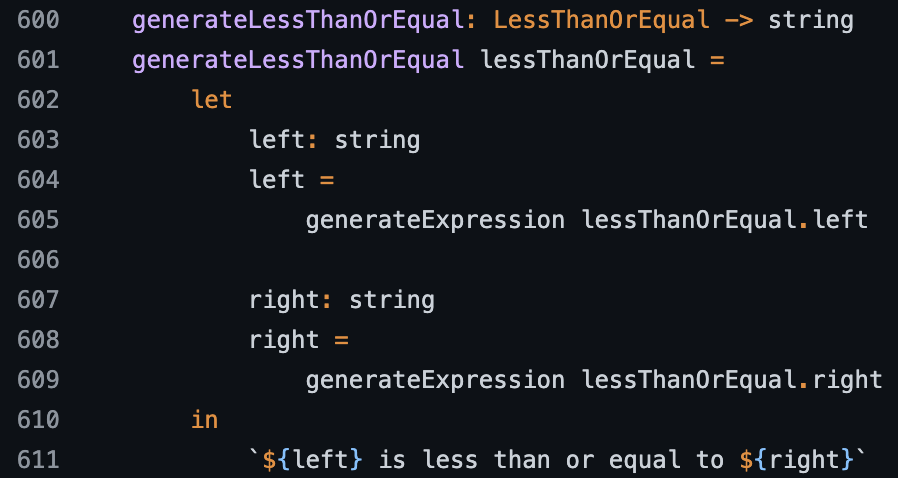
\includegraphics[scale=0.7]{assets/derwLTE.png}
    \caption[]{An excerpt from the english generator in Derw, showing how expressions with ``less than or equal'' are converted\footnotemark.}
    \label{fig:derw}
\end{figure}
\footnotetext{https://github.com/eeue56/derw/blob/main/src/generators/English.derw}

Another example is Pandoc, which works with markdown languages. It has a ``core language'' which all parsers and writers must work with:

\begin{verbatim}
    Plain [Inline]
    Para [Inline]
    LineBlock [[Inline]]
    CodeBlock Attr String
    RawBlock Format String
    BlockQuote [Block]
    OrderedList ListAttributes [[Block]]
    BulletList [[Block]]
    DefinitionList [([Inline], [[Block]])]
    Header Int Attr [Inline]
    HorizontalRule
    Table [Inline] [Alignment] [Double] [TableCell] [[TableCell]]
    Div Attr [Block]
    Null
\end{verbatim}

% [kilde]

Every inputlanguage must be able to parse to (at least) these data types, and every writer must be able to work with these data types. However, writing a document in a rich format like Latex, and later converting it to a different markup language might tends to pose problems due to the different philosophies that underlie each language. Yet Pandoc is an excellent interpreter of lightweight markup languages like Markdown, which are ``neutural'' by design \cite{dominici2014}.

\subsection{Haskell's strengths}
As previously mentioned, we opted for the Haskell programming language when implementing Psnodig. There are several reasons as to why, but the primary one is that it is widely perceived as a fitting tool when working with programming languages, and particularly when working with interpreters\footnote{https://github.com/Gabriella439/post-rfc/blob/main/sotu.md\#compilers}. At the end of the day, programming languages are just tools, and we believe this is the best one for this particular job. \hfill \\

With Haskell, it is straightforward to create your own \textbf{data types}, which are then used to model abstract syntax trees (ASTs). For instance, we can create our own calculator language in just a few lines of code:

\begin{verbatim}
    data Program = Program Expression

    data Expression =
          CompoundExpression Integer Operator Expression
        | IntExpression Integer

    data Operator =
          Plus
        | Minus
        | Times
        | Division
\end{verbatim}

From this, we can construct the following AST:

\begin{verbatim}
    Program (CompoundExpression 1 Plus
                (CompoundExpression 2 Minus
                    (IntExpression 3))
\end{verbatim}

As you can also see, we could create much bigger calculations than this, and if we wish to include extra operators, like for instance exponents in the future, we simply add a \texttt{| Exponent} to the Operator data type. \hfill \\

Another benefit of using Haskell, is that its strong type system opens for clean and efficient pattern matching. This is very useful, both when writing the interpreter, but also when adding new, potential readers. For instance, if we wish to transpile the above AST to text, we could start with writing a function to convert the operators:

\begin{lstlisting}[caption={Haskell example to convert data type to string}, captionpos=b]
    f :: Operator -> String
    f (Operator Plus)     = " + "
    f (Operator Minus)    = " - "
    f (Operator Times)    = " / "
    f (Operator Division) = " * "
\end{lstlisting}

The function \textbf{f} takes something of type \textbf{Operator} as input, and returns something of type \textbf{String}. It will pattern match on the input, and return a correspondng value, making it bijective. We could add case of \texttt{f \_ = ""}, which would return the empty string for any other kind of operator, though this would be redundant as we have not defined any other type of operator anyway. \hfill \\

Lastly, we can utilise the QuickCheck\footnote{https://hackage.haskell.org/package/QuickCheck}, which is a testing library suited for automatic property-based testing in Haskell. With this we can prove different properties of our tool \cite{DBLP:conf/icfp/ClaessenH00}, and perhaps also of other (primarily) parsers and (maybe) writers, given that they have to pass through Haskell ADTs anyway.